\documentclass{article}
\usepackage{graphicx}
\usepackage{listings}
\usepackage{color}
\usepackage{float}
\usepackage{tikz}
\usetikzlibrary{shapes, arrows, positioning}

\title{Practical Work 2: RPC File Transfer}
\author{Nguyen Thanh Dat \\ Student ID: 23BI14091}
\date{}%
\begin{document}
\maketitle
\section{Introduction}
The goal of this practical work is to upgrade the previous TCP file transfer system to use \textbf{Remote Procedure Call (RPC)}. 
Unlike the previous implementation, which handled raw socket streams and data chunking manually, this system abstracts the networking layer, allowing the client to invoke a function on the server as if it were local.

\section{RPC Service Design}
To implement file transfer, I designed a specific RPC function that is exposed by the server. 
Instead of defining a packet protocol (headers, delimiters, etc.), I defined a service interface.

\subsection{Service Definition}
The server registers a single function:
\begin{itemize}
    \item \textbf{Function Name:} \texttt{save\_file(filename, binary\_data)}
    \item \textbf{Input:} A string representing the name of the file and a binary object containing the file's raw bytes.
    \item \textbf{Output:} Returns \texttt{True} if the write operation was successful.
\end{itemize}

\subsection{Interaction Diagram}
The interaction is synchronous. The client reads the file, wraps it, and calls the remote method.

\begin{figure}[H]
    \centering
    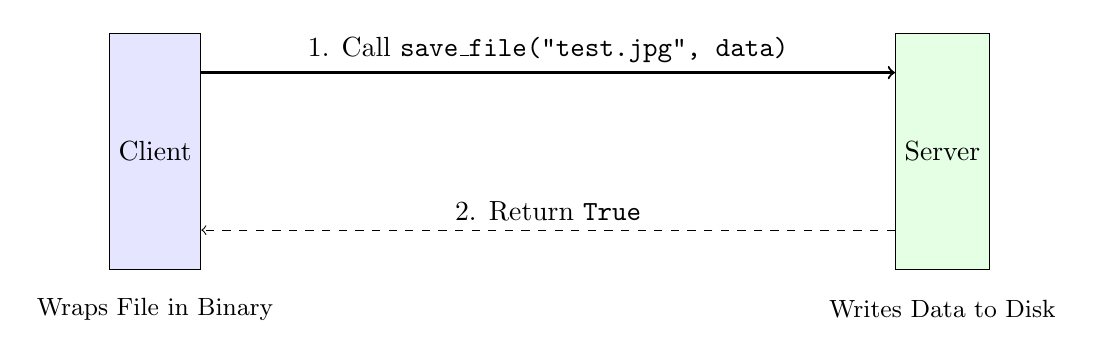
\begin{tikzpicture}[node distance=10cm, auto]
        % Nodes
        \node (client) [draw, rectangle, minimum height=3cm, fill=blue!10] {Client};
        \node (server) [draw, rectangle, minimum height=3cm, fill=green!10, right of=client] {Server};
        
        % Arrows
        \draw[->, thick] ([yshift=1cm]client.east) -- node[above] {1. Call \texttt{save\_file("test.jpg", data)}} ([yshift=1cm]server.west);
        \draw[->, dashed] ([yshift=-1cm]server.west) -- node[above] {2. Return \texttt{True}} ([yshift=-1cm]client.east);
        
        % Internal logic labels
        \node[below of=client, node distance=2cm] {\small Wraps File in Binary};
        \node[below of=server, node distance=2cm] {\small Writes Data to Disk};
    \end{tikzpicture}
    \caption{Sequence Diagram of the RPC Call}
    \label{fig:sequence}
\end{figure}

\section{System Organization}
The system leverages Python's built-in \texttt{xmlrpc} library.
\begin{itemize}
    \item \textbf{Server Side:} Uses \texttt{SimpleXMLRPCServer} to listen on a specific port and register the \texttt{save\_file} function.
    \item \textbf{Client Side:} Uses \texttt{ServerProxy} to create a local stub that forwards calls to the server over HTTP/XML.
\end{itemize}

\begin{figure}[H]
    \centering
    \resizebox{\textwidth}{!}{ 
    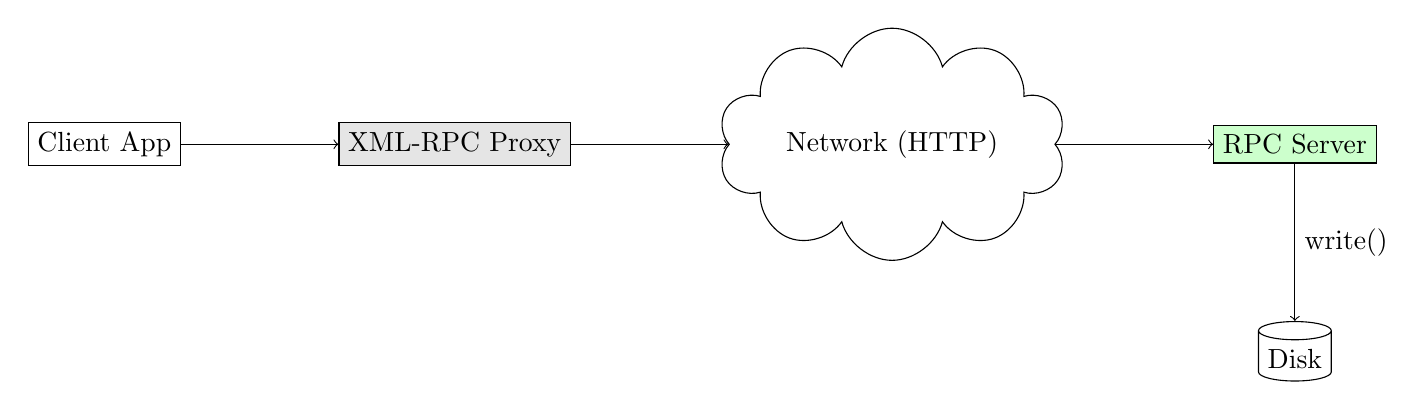
\begin{tikzpicture}[node distance=2cm]
        \node (client) [draw, rectangle] {Client App};
        \node (proxy) [draw, rectangle, right=of client, fill=gray!20] {XML-RPC Proxy};
        \node (network) [cloud, draw, right=of proxy, aspect=2, fill=white] {Network (HTTP)};
        \node (server) [draw, rectangle, right=of network, fill=green!20] {RPC Server};
        \node (disk) [draw, cylinder, shape border rotate=90, aspect=0.25, below=of server] {Disk};

        \draw[->] (client) -- (proxy);
        \draw[->] (proxy) -- (network);
        \draw[->] (network) -- (server);
        \draw[->] (server) -- node[right] {write()} (disk);
    \end{tikzpicture}
    }
    \caption{System Architecture}
    \label{fig:arch}
\end{figure}

\section{Implementation}

\subsection{Server Implementation}
The server defines the logic to unwrap the binary data and write them to a file.

\begin{lstlisting}[language=Python, basicstyle=\small, breaklines=true, frame=single]
import os
from xmlrpc.server import SimpleXMLRPCServer

def save_file(filename, file_data):
    print(f"Receiving file: {filename}...")
    try:
        # Access .data to get raw bytes from XMLRPC Binary object
        with open("received_" + filename, "wb") as handle:
            handle.write(file_data.data)
        return True
    except Exception as e:
        return False

# Registration
server = SimpleXMLRPCServer(('127.0.0.1', 65432))
server.register_function(save_file, "save_file")
server.serve_forever()
\end{lstlisting}

\subsection{Client Implementation}
The client manages the reading of files and the calls to remote procedures.

\begin{lstlisting}[language=Python, basicstyle=\small, breaklines=true, frame=single]
import xmlrpc.client

proxy = xmlrpc.client.ServerProxy('http://127.0.0.1:65432')

with open("test.jpg", "rb") as handle:
    # Wrap raw bytes for XML-RPC transfer
    binary_data = xmlrpc.client.Binary(handle.read())

proxy.save_file("test.jpg", binary_data)
\end{lstlisting}

\section{Verification}
The following screenshot illustrates the successful execution of the client script and the server's acknowledgement.

\begin{figure}[H]
\centering
\includegraphics[width=0.9\textwidth]{screenshot.png}
\caption{Successful File Transfer Execution}
\end{figure}

\end{document}